
\documentclass[11pt,compress,t,notes=noshow, xcolor=table]{beamer}
\usepackage[]{graphicx}\usepackage[]{color}
% maxwidth is the original width if it is less than linewidth
% otherwise use linewidth (to make sure the graphics do not exceed the margin)
\makeatletter
\def\maxwidth{ %
  \ifdim\Gin@nat@width>\linewidth
    \linewidth
  \else
    \Gin@nat@width
  \fi
}
\makeatother

\definecolor{fgcolor}{rgb}{0.345, 0.345, 0.345}
\newcommand{\hlnum}[1]{\textcolor[rgb]{0.686,0.059,0.569}{#1}}%
\newcommand{\hlstr}[1]{\textcolor[rgb]{0.192,0.494,0.8}{#1}}%
\newcommand{\hlcom}[1]{\textcolor[rgb]{0.678,0.584,0.686}{\textit{#1}}}%
\newcommand{\hlopt}[1]{\textcolor[rgb]{0,0,0}{#1}}%
\newcommand{\hlstd}[1]{\textcolor[rgb]{0.345,0.345,0.345}{#1}}%
\newcommand{\hlkwa}[1]{\textcolor[rgb]{0.161,0.373,0.58}{\textbf{#1}}}%
\newcommand{\hlkwb}[1]{\textcolor[rgb]{0.69,0.353,0.396}{#1}}%
\newcommand{\hlkwc}[1]{\textcolor[rgb]{0.333,0.667,0.333}{#1}}%
\newcommand{\hlkwd}[1]{\textcolor[rgb]{0.737,0.353,0.396}{\textbf{#1}}}%
\let\hlipl\hlkwb

\usepackage{framed}
\makeatletter
\newenvironment{kframe}{%
 \def\at@end@of@kframe{}%
 \ifinner\ifhmode%
  \def\at@end@of@kframe{\end{minipage}}%
  \begin{minipage}{\columnwidth}%
 \fi\fi%
 \def\FrameCommand##1{\hskip\@totalleftmargin \hskip-\fboxsep
 \colorbox{shadecolor}{##1}\hskip-\fboxsep
     % There is no \\@totalrightmargin, so:
     \hskip-\linewidth \hskip-\@totalleftmargin \hskip\columnwidth}%
 \MakeFramed {\advance\hsize-\width
   \@totalleftmargin\z@ \linewidth\hsize
   \@setminipage}}%
 {\par\unskip\endMakeFramed%
 \at@end@of@kframe}
\makeatother

\definecolor{shadecolor}{rgb}{.97, .97, .97}
\definecolor{messagecolor}{rgb}{0, 0, 0}
\definecolor{warningcolor}{rgb}{1, 0, 1}
\definecolor{errorcolor}{rgb}{1, 0, 0}
\newenvironment{knitrout}{}{} % an empty environment to be redefined in TeX

\usepackage{alltt}
\newcommand{\SweaveOpts}[1]{}  % do not interfere with LaTeX
\newcommand{\SweaveInput}[1]{} % because they are not real TeX commands
\newcommand{\Sexpr}[1]{}       % will only be parsed by R
\newcommand{\xmark}{\ding{55}}%


\usepackage[english]{babel}
\usepackage[utf8]{inputenc}

\usepackage{dsfont}
\usepackage{verbatim}
\usepackage{amsmath}
\usepackage{amsfonts}
\usepackage{amssymb}
\usepackage{bm}
\usepackage{csquotes}
\usepackage{multirow}
\usepackage{longtable}
\usepackage{booktabs}
\usepackage{enumerate}
\usepackage[absolute,overlay]{textpos}
\usepackage{psfrag}
\usepackage{algorithm}
\usepackage{algpseudocode}
\usepackage{eqnarray}
\usepackage{arydshln}
\usepackage{tabularx}
\usepackage{placeins}
\usepackage{tikz}
\usepackage{setspace}
\usepackage{colortbl}
\usepackage{mathtools}
\usepackage{wrapfig}
\usepackage{bm}
\usepackage{amsmath}
\usepackage{pifont}
\usepackage{xcolor} %colored math symbols

\usetikzlibrary{shapes,arrows,automata,positioning,calc,chains,trees, shadows}
\tikzset{
  %Define standard arrow tip
  >=stealth',
  %Define style for boxes
  punkt/.style={
    rectangle,
    rounded corners,
    draw=black, very thick,
    text width=6.5em,
    minimum height=2em,
    text centered},
  % Define arrow style
  pil/.style={
    ->,
    thick,
    shorten <=2pt,
    shorten >=2pt,}
}

\usepackage{subfig}

% Defines macros and environments
\usepackage{../../style/lmu-lecture}


\let\code=\texttt
\let\proglang=\textsf

\setkeys{Gin}{width=0.9\textwidth}

\setbeamertemplate{frametitle}{\expandafter\uppercase\expandafter\insertframetitle}

\usepackage{bbm}
% basic latex stuff
\newcommand{\pkg}[1]{{\fontseries{b}\selectfont #1}} %fontstyle for R packages
\newcommand{\lz}{\vspace{0.5cm}} %vertical space
\newcommand{\dlz}{\vspace{1cm}} %double vertical space
\newcommand{\oneliner}[1] % Oneliner for important statements
{\begin{block}{}\begin{center}\begin{Large}#1\end{Large}\end{center}\end{block}}


%new environments
\newenvironment{vbframe}  %frame with breaks and verbatim
{
 \begin{frame}[containsverbatim,allowframebreaks]
}
{
\end{frame}
}

\newenvironment{vframe}  %frame with verbatim without breaks (to avoid numbering one slided frames)
{
 \begin{frame}[containsverbatim]
}
{
\end{frame}
}

\newenvironment{blocki}[1]   % itemize block
{
 \begin{block}{#1}\begin{itemize}
}
{
\end{itemize}\end{block}
}

\newenvironment{fragileframe}[2]{  %fragile frame with framebreaks
\begin{frame}[allowframebreaks, fragile, environment = fragileframe]
\frametitle{#1}
#2}
{\end{frame}}


\newcommand{\myframe}[2]{  %short for frame with framebreaks
\begin{frame}[allowframebreaks]
\frametitle{#1}
#2
\end{frame}}

\newcommand{\remark}[1]{
  \textbf{Remark:} #1
}


\newenvironment{deleteframe}
{
\begingroup
\usebackgroundtemplate{
\includegraphics[width=\paperwidth,height=\paperheight]{../style/color/red.png}}
 \begin{frame}
}
{
\end{frame}
\endgroup
}
\newenvironment{simplifyframe}
{
\begingroup
\usebackgroundtemplate{
\includegraphics[width=\paperwidth,height=\paperheight]{../style/color/yellow.png}}
 \begin{frame}
}
{
\end{frame}
\endgroup
}\newenvironment{draftframe}
{
\begingroup
\usebackgroundtemplate{
\includegraphics[width=\paperwidth,height=\paperheight]{../style/color/green.jpg}}
 \begin{frame}
}
{
\end{frame}
\endgroup
}
% https://tex.stackexchange.com/a/261480: textcolor that works in mathmode
\makeatletter
\renewcommand*{\@textcolor}[3]{%
  \protect\leavevmode
  \begingroup
    \color#1{#2}#3%
  \endgroup
}
\makeatother


\input{../../latex-math/basic-math}
\input{../../latex-math/basic-ml}
\input{../../latex-math/ml-nn}

\newcommand{\titlefigure}{plots/architectures/lenet.png}
%modify picture
\newcommand{\learninggoals}{
  \item LeNet
  \item AlexNet
  \item VGG
  \item Network in Network
}

\title{Deep Learning}
\date{}



\begin{document}

\lecturechapter{Modern Architectures - I}
\lecture{I2DL}
%%%%%%%%%%%%%%%%%%%%%%%%%%%%%%%%%%%%%%%%%%%%%%%%%%%%%%%%%%%%%%%%%%
%\section{From LeNet to AlexNet}

\section{LeNet}

\begin{vbframe}{LeNet Architecture}
  \begin{itemize}
    \item Pioneering work on CNNs by Yann Lecun in 1998. 
    \item Applied on the MNIST dataset for automated handwritten digit recognition.
    \item Consists of convolutional, "subsampling" and dense layers.
    \item Complexity and depth of the net was mainly restricted by limited computational power back in the days.
  \end{itemize}
  \begin{figure}
  \centering
    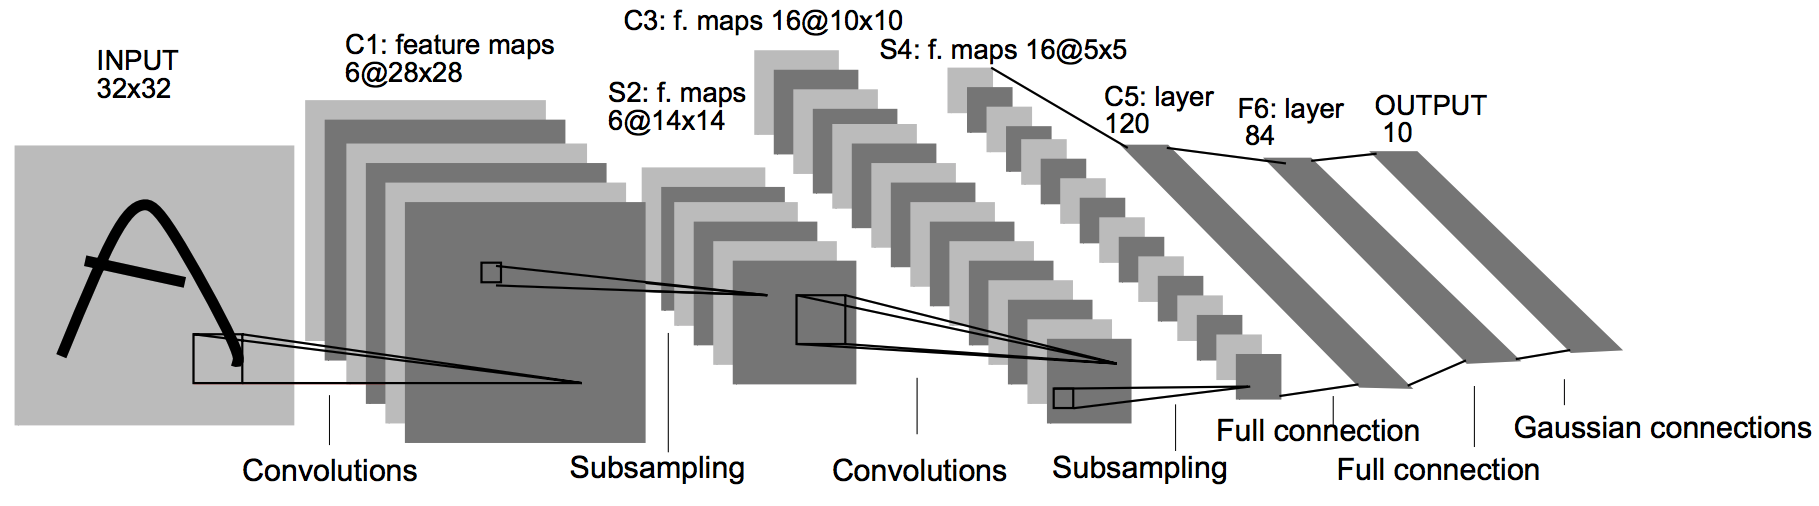
\includegraphics[width=9cm]{plots/architectures/lenet.png}
    \caption{LeNet architecture: two conv layers with subsampling, followed by dense layers and a 'Gaussian connections' layer.}
  \end{figure}
  \framebreak
  \begin{itemize}
    \item A neuron in a subsampling layer looks at a $2 \times 2$ region of a feature map, sums the four values, multiplies it by a trainable coefficient, adds a trainable bias and then applies a sigmoid activation.
    \item A stride of 2 ensures that the size of the feature map reduces by about a half.
    \item The 'Gaussian connections' layer has a neuron for each possible class. 
    \item The output of each neuron in this layer is the (squared) Euclidean distance between the activations from the previous layer and the weights of the neuron.
  \end{itemize}   
\end{vbframe}

\section{AlexNet}
\begin{vbframe}{AlexNet}
  \begin{itemize}
    \item AlexNet, which employed an 8-layer CNN, won the ImageNet Large Scale Visual Recognition (LSVR) Challenge 2012 by a phenomenally large margin.
    \item The network trained in parallel on two small GPUs, using two streams of convolutions which are partly interconnected.
    \item The architectures of AlexNet and LeNet are very similar, but there are also significant differences: 
       \begin{itemize}
          \item First, AlexNet is deeper than the comparatively small LeNet5. AlexNet consists of eight layers: five convolutional layers, two fully-connected hidden layers, and one fully-connected output layer. 
          \item Second, AlexNet used the ReLU instead of the sigmoid as its activation function. 
       \end{itemize}
  \end{itemize}
    \begin{figure}
        \centering
        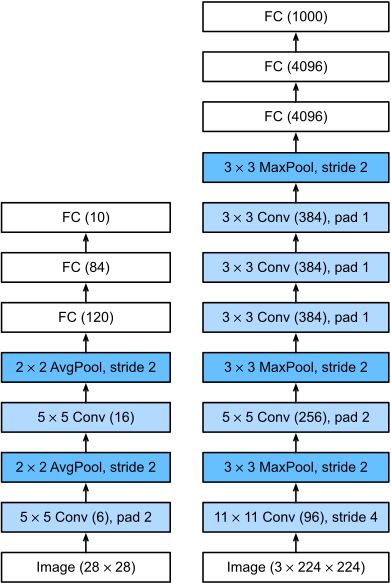
\includegraphics[width=4.5cm]{plots/moderncnn/alexnet.png}
        \caption{From LeNet (left) to AlexNet (right).}
    \end{figure}
\end{vbframe}


%%%%%%%%%%%%%%%%%%%%%%%%%%%%%%%%%%%%%%%%%%%%%%%%%%%%%%%%%%%%%%%%%%
\section{VGG}

%\subsection{VGG Blocks}
\begin{vbframe}{VGG Blocks}
  \begin{itemize}
    \item The block composed of convolutions with $3 \times 3$  kernels with padding of 1 (keeping height and width) and $2 \times 2$  max pooling with stride of 2 (halving the resolution after each block).
    \item The use of blocks leads to very compact representations of the network definition. 
    \item It allows for efficient design of complex networks.
  \end{itemize}
  
    \begin{figure}
  \centering
    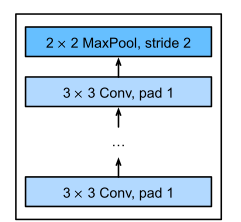
\includegraphics[width=3cm]{plots/moderncnn/vggblock.png}
    \tiny{\\ credit : D2DL}
    \caption{VGG block.}
  \end{figure}
  
\end{vbframe}


%\subsection{VGG Network}

\begin{vbframe}{VGG Network}
  \begin{itemize}
    \item Architecture introduced by Simonyan and Zisserman, 2014 as \enquote{Very Deep Convolutional Network}.
    \item A deeper variant of the AlexNet.
    \item Basic idea is to have small filters and Deeper networks
    \item Mainly uses many cnn layers with a small kernel size $3 \times 3$.
    \item Stack of three $3 \times 3$ cnn (stride 1) layers has same effective receptive field as one $7 \times 7$ conv layer.
    \item Performed very well in the ImageNet Challenge in 2014.
    \item Exists in a small version (VGG16) with a total of 16 layers (13 cnn layers and 3 fc layers) and 5 VGG blocks while a larger version (VGG19) with 19 layers (16 cnn layers and 3 fc layers) and 6 VGG blocks.
  \end{itemize}
\framebreak
  \begin{figure}
  \centering
    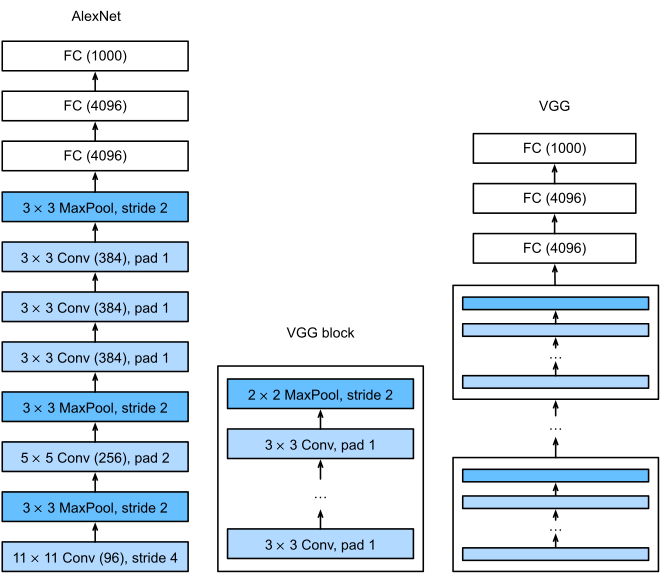
\includegraphics[width=7cm]{plots/moderncnn/vgg.png}
    \tiny{\\ credit : D2DL}
    \caption{From AlexNet to VGG that is designed from building blocks.}
  \end{figure}

\end{vbframe}

\section{Network in Network (NiN)}


\begin{vbframe}{NiN Blocks}
  \begin{itemize}
    \item The idea behind NiN is to apply a fully-connected layer at each pixel location (for each height and width). If we tie the weights across each spatial location, we could think of this as a $1 \times 1$ convolutional layer.
    \item The NiN block consists of one convolutional layer followed by two $1 \times 1$  convolutional layers that act as per-pixel fully-connected layers with ReLU activations.
    \item The convolution window shape of the first layer is typically set by the user. The subsequent window shapes are fixed to $1 \times 1$.
  \end{itemize}
  \begin{figure}
  \centering
    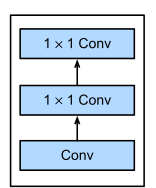
\includegraphics[width=2cm]{plots/moderncnn/ninblock.png}
    \tiny{\\ credit : D2DL}
    \caption{NiN block.}
  \end{figure}

\end{vbframe}


\begin{vbframe}{Global average pooling}
    \begin{itemize}
        \item Problem setting: tackle overfitting in the final fully connected layer.
        \begin{itemize}
        \item Classic pooling removes spatial information and is mainly used for dimension and parameter reduction.
        \item The elements of the final feature maps are connected to the output layer via a dense layer. This could require a huge number of weights increasing the danger of overfitting.
        \item Example: 256 feature maps of dim 100x100 connected to 10 output neurons lead to $256\times 10^5$ weights for the final dense layer.
        \end{itemize}
        

\framebreak 

        \item Solution: 
        \begin{itemize}
            \item Average each final feature map to the element of one global average pooling (GAP) vector.
            \item Example: 256 feature maps are now reduced to GAP-vector of length 256 yielding a final dense layer with 2560 weights.
        \end{itemize}
    \end{itemize}

    \begin{figure}
        \centering
        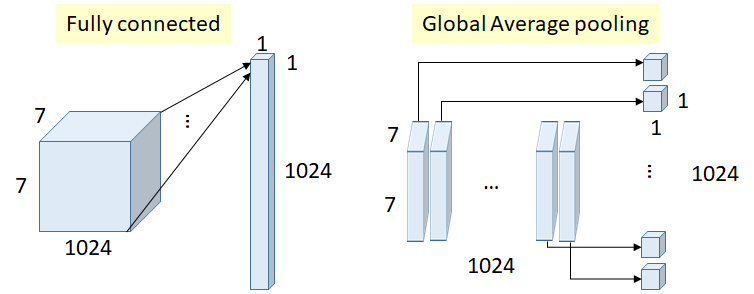
\includegraphics[width=8cm]{plots/moderncnn/GAP.png}
        \small{\caption{An Example of Fully Connected Layer VS Global Average Pooling Layer}}
    \end{figure}

\framebreak

    \begin{itemize}
        \item GAP preserves whole information from the single feature maps whilst decreasing the dimension.
        \item Mitigates the possibly \textbf{destructive} effect of pooling.
        \item Each element of the GAP output represents the activation of a certain feature on the input data.
        \item Acts as an additional regularizer on the final fully connected layer.
    \end{itemize}

\end{vbframe}


\begin{vbframe}{Network in Network (NiN)}
  \begin{itemize}
    \item NiN uses blocks consisting of a convolutional layer and multiple $1 \times 1$ convolutional layers. This can be used within the convolutional stack to allow for more per-pixel nonlinearity.
    \item NiN removes the fully-connected layers and replaces them with global average pooling (i.e., summing over all locations) after reducing the number of channels to the desired number of outputs (e.g., 10 for Fashion-MNIST).
    \item Removing the fully-connected layers reduces overfitting. NiN has dramatically fewer parameters.
    \item The NiN design influenced many subsequent CNN designs.
  \end{itemize}
\framebreak
  \begin{figure}
  \centering
    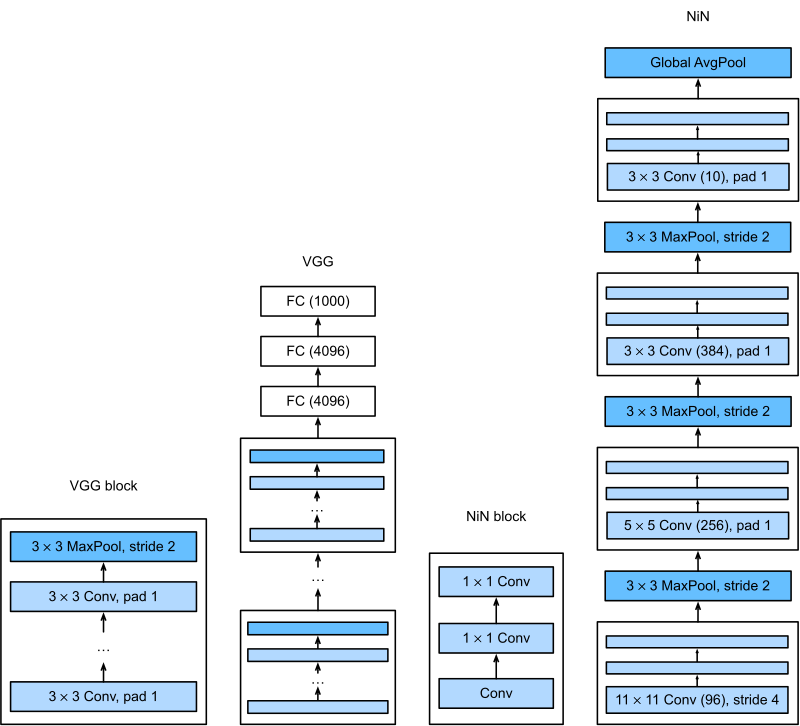
\includegraphics[width=7cm]{plots/moderncnn/nin.png}
    \tiny{\\ credit : D2DL}
    \caption{Comparing architectures of VGG and NiN, and their blocks.}
  \end{figure}

\end{vbframe}


%%%%%%%%%%%%%%%%%%%%%%%%%%%%%%%%%%%%%%%%%%%%%%%%%%%%%%%%%%%%%%%%%%


%%%%%%%%%%%%%%%%%%%%%%%%%%%%%%%%%%%%%%%%%%%%%%%%%%%%%%%%%%%%%%%%%%
%%%%%%%%%%%%%%%%%%%%%%%%%%%%%%%%%%%%%%%%%%%%%%%%%%%%%%%%%%%%%%%%%%

%%%%%%%%%%%%%%%%%%%%%%%%%%%%%%%%%%%%%%%%%%%%%%%%%%%%%%%%%%%%%%%%%%
%%%%%%%%%%%%%%%%%%          REFERENCES          %%%%%%%%%%%%%%%%%%
%%%%%%%%%%%%%%%%%%%%%%%%%%%%%%%%%%%%%%%%%%%%%%%%%%%%%%%%%%%%%%%%%%
\begin{vbframe}
\frametitle{References}
\footnotesize{
\begin{thebibliography}{99}

% \bibitem[Ronneberger et al., 2015]{12} Olaf Ronneberger, Philipp Fischer, Thomas Brox (2015)
% \newblock U-Net: Convolutional Networks for Biomedical Image Segmentation
% \newblock \emph{\url{http://arxiv.org/abs/1505.04597}}
% %%%%%%%%%%%%%%%%%%%%%%%%%%%%%%%%%%
\bibitem[Zhou et. al , 2016]{25} B. Zhou, Khosla, A., Labedriza, A., Oliva, A. and A. Torralba (2016)
\newblock Deconvolution and Checkerboard Artifacts
\newblock \emph{\url{http://cnnlocalization.csail.mit.edu/Zhou_Learning_Deep_Features_CVPR_2016_paper.pdf}}
%%%%%%%%%%%%%%%%%%%%%%%%%%%%%%%%%%
%%%%%%%%%%%%%%%%%%%%%%%%%%%%%%%%%%
\bibitem[Szegedy et. al , 2014]{26} Christian Szegedy, Wei Liu, Yangqing Jia, Pierre Sermanet, Scott Reed, Dragomir Anguelov, Dumitru Erhan, Vincent Vanhoucke and Andrew Rabinovich (2014)
\newblock Going deeper with convolutions
\newblock \emph{\url{https://arxiv.org/abs/1409.4842}}
%%%%%%%%%%%%%%%%%%%%%%%%%%%%%%%%%%
%%%%%%%%%%%%%%%%%%%%%%%%%%%%%%%%%%
% \bibitem[Jie Hu et. al , 2014]{27} Jie Hu, Shen, Li and Gang Sun (2017)
% \newblock Squeeze-and-Excitation Networks
% \newblock \emph{\url{https://arxiv.org/abs/1709.01507}}
%%%%%%%%%%%%%%%%%%%%%%%%%%%%%%%%%%
%%%%%%%%%%%%%%%%%%%%%%%%%%%%%%%%%%
% \bibitem[Szegedy Christian et. al , 2015]{28} Christian Szegedy, Vanhoucke, Vincent, Sergey, Ioffe, Shlens, Jonathan and Wojna Zbigniew (2015)
% \newblock Rethinking the Inception Architecture for Computer Vision
% \newblock \emph{\url{https://arxiv.org/abs/1512.00567}}
%%%%%%%%%%%%%%%%%%%%%%%%%%%%%%%%%%
%%%%%%%%%%%%%%%%%%%%%%%%%%%%%%%%%%
\bibitem[He et. al , 2015]{29} Kaiming He, Zhang, Xiangyu, Ren, Shaoqing, and Jian Sun (2015)
\newblock Deep Residual Learning for Image Recognition
\newblock \emph{\url{https://arxiv.org/abs/1512.03385}}
%%%%%%%%%%%%%%%%%%%%%%%%%%%%%%%%%%
%%%%%%%%%%%%%%%%%%%%%%%%%%%%%%%%%%
\bibitem[Zhou et. al, 2016]{32} Bolei Zhou, Aditya Khosla, Agata Lapedriza, Aude Oliva and Antonio Torralba (2016)
\newblock Learning Deep Features for Discriminative Localization
\newblock \emph{\url{http://cnnlocalization.csail.mit.edu/Zhou_Learning_Deep_Features_CVPR_2016_paper.pdf}}
%%%%%%%%%%%%%%%%%%%%%%%%%%%%%%%%%%
%%%%%%%%%%%%%%%%%%%%%%%%%%%%%%%%%%



\end{thebibliography}
}
\end{vbframe}
%%%%%%%%%%%%%%%%%%%%%%%%%%%%%%%%%%%%%%%%%%%%%%%%%%%%%%%%%%%%%%%%%%
%%%%%%%%%%%%%%%%%%%%%%%%%%%%%%%%%%%%%%%%%%%%%%%%%%%%%%%%%%%%%%%%%%
\endlecture
\end{document}
